%versi 2 (8-10-2016)
\chapter{Landasan Teori}
\label{chap:teori}
\setcounter{secnumdepth}{3}
\section{Codeigniter}
\label{sec:codeigniter} 
 
Codeigniter adalah \textit{framework} pengembangan aplikasi untuk \textit{developer} yang membangun situs web menggunakan PHP. Tujuannya adalah untuk memungkinkan Anda mengembangkan proyek lebih cepat, daripada bila \textit{developer} menulis kode dari awal, dengan menyediakan banyak kumpulan \textit{library} untuk tugas-tugas yang sering dibutuhkan dan juga menyediakan tampilan sederhana serta struktur logika untuk mengakses \textit{library-library} tersebut. Codeigniter memungkinkan \textit{developer} untuk fokus secara kretif pada proyek \textit{developer} dengan cara meminimalkan jumlah kode yang dibutuhkan untuk setiap tugas yang diberikan. \cite{codeigniter:17}
\\
\\
Codeigniter dirancang untuk memenuhi kebutuhan :
\begin{itemize}
		\item \textit{Framework} dengan tapak keberadaan yang kecil
		\item performa yang baik
		\item kompabilitas akun \textit{hosting} yang luas yang dapat berjalan di berbagai versi dan konfigurasi PHP
		\item \textit{Framework} yang hampir tidak membutuhkan konfigurasi
		\item \textit{Framework} yang tidak membutuhkan \textit{command line}
		\item \textit{Framework} yang tidak mengikuti aturan pengkodean yang ketat
		\item membutuhkan solusi yang sederhana
		\item dokumentasi yang menyeluruh
	\end{itemize}
	
\subsection{Model-View-Controller}
Codeigniter didasari pola pengembangan \textit{Model-View-Controller} atau MVC. MVC memisahkan logika aplikasi dengan tampilannya.

\begin{itemize}
		\item \textbf{\textit{Model}} merepresentasikan struktur data. Pada umumnya kelas-kelas model menampung fungsi-fungsi untuk mengambil, memperbarui atau memasukan data ke dalam basis data.
		\item \textbf{\textit{View}} menampilkan informasi ke pengguna. 
		\item \textbf{\textit{Controller}} berfungsi sebagai perantara antara model dan view.
\end{itemize}

\subsection{Controller}
Sebuah \textit{controller} adalah kelas yang dinamakan demikian agar dapat diasosiasikan dengan URI.
sebagai contoh URI "example.com/index.php/blog/" , Codeigniter akan mencari controller bernama blog.php dan menjalankannya.

	\subsubsection{Method}
	Untuk menjalankan suatu method, maka developer perlu menuliskannya pada segmen kedua URI. Contoh "example.com/index.php/blog/comments" maka akan dijalankan method comments() pada controller blog.php. Method yang akan dijalankan bila bagian kedua URI kosong adalah method index(). Jika URI mengandung lebih dari dua segment, segment-segment tersebut akan dimasukan ke dalam method sebagai parameter.
	
	\subsubsection{Default Controller}
	Codeigniter dapat diperintahkan untuk menjalankan \textit{default controller} jika tidak terdapat URI, pada umumnya terjadi ketika hanya terdapat permintaan menggunakan URL dasar \textit{website}. Penentuan \textit{default controller} terdapat pada \textit{file} "application/config/routes.php" dan set variabel . Nama \textit{controller} tersebut adalah 'blog', maka ketika index.php dijalankan tanpa menspesifikasikan URI akan dijalankan \textit{controller} 'blog'.

\subsection{View}
\textit{View} adalah sebuah halaman web, bagian-bagian halaman ( seperti \textit{header, footer, sidebar}, dan-lain-lain) atau bagian dari \textit{view} lainnya. \textit{View} tidak pernah dipanggil secara langsung, melainkan harus melalui controller karena dalam framework MVC controller berfungsi sebagai pengatur.

\subsection{Model}
Model adalah kelas PHP yang dirancang untuk bekerja dengan informasi-informasi di \textit{database}. Sebagai contoh, misalkan codeigniter digunakan untuk mengatur sebuah blog maka model mengandung fungsi-fungsi seperti \textit{select, insert, update }data-data blog.

\subsubsection{Anatomi dari Model}
Model disimpan di direktori \textbf{application/models}. Model dapat disimpan dalam sub-direktori jika dibutuhkan. Bentuk dasar kode pada kelas model adalah seperti di bawah ini:
\begin{lstlisting}
	class Model_name extends CI_Model {
	
		public function_construct()
		{
			parent::_construct();
			//constructor code
		}
	}
\end{lstlisting}
\textbf{Model\_name} adalah nama dari kelasnya. Huruf pertama dari nama kelas harus huruf kapital dengan huruf-huruf setelahnya ditulis menggunakan huruf kecil. Kelas model harus dipastikan meng-\textit{extend} kelas Model dasar. Nama file harus sama dengan nama kelasnya.

\subsubsection{Load Model}
Pada umumnya model akan di-\textit{load} di dalam method-method \textit{controller}. Untuk \textit{load} model diperlukan method berikut:
\begin{lstlisting}
	$this->model->model('model_name');
\end{lstlisting}
Jika model terdapat pada sub-direktori, perlu dimasukan \textit{path}-nya ke dalam direktori 'models'. Misalnya model terdapat di \textit{application/models/blog/Queries.php} maka untuk \textit{load} model digunakan :
\begin{lstlisting}
	$this->load->model('blog/queries');
\end{lstlisting}


\subsection{Flow Chart Codeignter}
Gambar dibawah mengilustrasikan aliran data dalam sistem : \footnote{https://www.codeigniter.com/userguide3/overview/appflow.html}
\begin{figure} [H]
	\centering  
	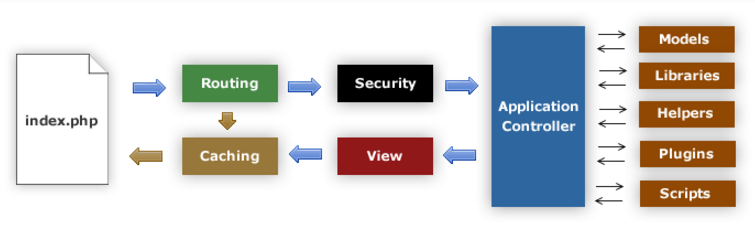
\includegraphics[scale=0.7]{appflowchart.png}  
	\caption[Flow Chart Codeignter]{Flow Chart Codeignter} 
	\label{fig:flow-chart-codeigniter} 
\end{figure}

\begin{enumerate}
		\item index.php berfungsi sebagai controller depan. Menginisialisasi sumber daya yang dibutuhkan untuk menjalankan Codeigniter
		\item Router memeriksa permintaan HTTP untuk menentukan apa yang akan dilakukan pada permintaan tersebut.
		\item Jika ada cache file, maka akan dikirim langsung ke browser. Melewati cara eksekusi sistem yang normal.
		\item Security. Sebelum controller aplikasi dimuat, permintaan HTTP dan data-data pengguna yang telah diserahkan disaring untuk kemanan.
		\item Controller memuat model, pustaka inti (\textit{core libraries}), pembantu dan sumber daya lain yang dibutuhkan untuk memproses permintaan khusus.
		\item Kemudian tampilan akhir dibuat dan dikirim ke web browser untuk dilihat. Jika caching diaktifkan, maka tampilan dimasukan ke dalam cache terlebih dahulu sehingga pada permintaan selanjutnya tampilan tersebut dapat diakses lebih cepat.
	\end{enumerate}


\section{Zurb Foundation}
\label{zurbfoundation}

\paragraph{}  Foundation adalah kumpulan pola desain HTML, CSS dan Javascript yang dapat digunakan untuk membuat website. Hal tersebut untuk membantu \textit{developer} agar tidak perlu menulis kode yang sama berulang kali. Selain membantu mengehemat waktu, Foundation juga membantu \textit{developer} untuk menulis kode dengan lebih baik. Foundation dapat bekerja pada berbagai media seperi komputer desktop, laptop, tablet, dan telepon genggam.\cite{zurbfoundation:17} 

Komponen-komponen dalam Foundation sendiri ada beberapa macam diantarnya sebagai berikut:\footnote{http://foundation.zurb.com/sites/docs/v/5.5.3/}

\begin{itemize}
	\item  Grid untuk mempermudah pembagian halaman
	\item  Desain tombol yang bermacam-macam. Desain tombol ini dapat diubah-ubah dengan cara menambahkan kelas.
	\item  Navigasi untuk mempermudah pengunjung aplikasi dalam menggunakan aplikasinya.
	\item  Plugins JavaScript untuk mempermudah \textit{developer} dalam membuat tampilan aplikasinya.
\end{itemize}


\section{Google OAuth 2.0} %https://developers.google.com/identity/protocols/OAuth2
\label{googleoauth}

\paragraph{} Google OAuth 2.0 merupakan salah satu protokol dari Google Sign-in. Google OAuth 2.0 digunakan oleh Google API untuk otorisasi dan autentikasi. Secara garis besar, cara pemakaian Google OAuth 2.0 adalah sebagai berikut : \footnote{https://developers.google.com/identity/protocols/OAuth2}

	\begin{enumerate}
  	\item Dapatkan OAuth 2.0 credential dari konsol Google API. OAuth 2.0 credential seperti client ID dan client secret yang diketahui oleh Google dan aplikasi pengguna, dapat didapatkan di halaman https://console.developers.google.com/ . 
  	\item Dapatkan token akses dari Google Authorization Server. Sebelum aplikasi dapat mengakses data pribadi menggunakan Google API, aplikasi tersebut harus mendapat token akses yang memberikan akses ke API. Satu token akses dapat memberikan berbagai macam akses ke banyak API. Variable parameter "\textit{scope}" mengendalikan kumpulan-kumpulan sumber daya dan operasi yang telah diperbolehkan untuk diakses oleh token akses. Selama masa permintaan token akses, aplikasi mengirimkan satu atau lebih nilai ke dalam parameter "\textit{scope}". Ada beberapa cara untuk melakukan permintaan, tergantung dari tipe aplikasi yang sedang dibuat. Sebagai contoh aplikasi JavaScript dapat meminta token akses menggunakan \textit{redirect} dari \textit{browser} yang mengarah ke Google, sementara aplikasi lain yang terinstall di dalam perangkat yang tidak memiliki browser menggunakan \textit{web service} untuk melakukan permintaan. Beberapa permintaan membutuhkan tahap autentikasi yang meminta pengguna untuk masuk ke akun Google mereka. Setelah masuk ke dalam akun, pengguna akan diminta jika mereka bersedia untuk memberikan izin ke aplikasi yang sedang melakukan permintaan tersebut.
  	\begin{figure} [H]
	\centering  
	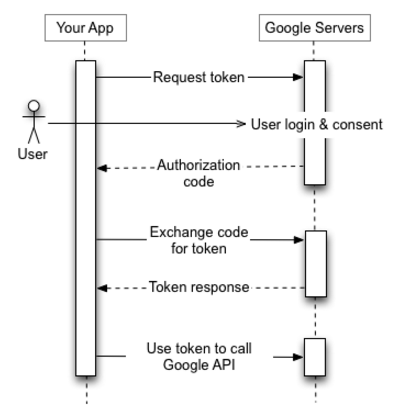
\includegraphics[scale=0.7]{skenario_token.png}  
	\caption[Skenario OAuth menggunakan token akses]{Skenario OAuth menggunakan token akses} 
	\label{fig:skenario-token} 
\end{figure}
  	\item Mengirim akses token ke API. Setelah aplikasi mendapatkan akses token, aplikasi tersebut akan mengirim token ke Google API dalam bentuk HTTP \textit{authorization header}. Jika memungkinkan, aplikasi dapat mengirim token-token sebagai parameter \textit{URI query-string}. Pengiriman dalam bentuk parameter URI tidak disarankan karena parameter URI dapat tersimpan dalam \textit{log} yang tidak aman. Token akses hanya berlaku untuk kumpulan operasi dan sumber daya yang dideskripsikan dalam parameter \textit{scope} di permintaan token. 
	\item Jika dibutuhkan, token akses dapat di-\textit{refresh} karena token akses memiliki masa berlaku terbatas. Jika aplikasi membutuhkan akses ke Google API lebih dari masa berlaku satu buah token, aplikasi dapat mendapatkan token \textit{refresh}. Token \textit{refresh} memungkinkan aplikasi untuk mendapatkan token akses baru.
  
\end{enumerate}

\section{PHPExcel} 
\label{phpexcel}

\paragraph{} PHPExcel adalah suatu proyek yang menyediakan berbagai kelas-kelas untuk pemrograman bahasa PHP yang memungkinkan \textit{developer} untuk menulis dan membaca dari berbagai macam bentuk \textit{spreadsheet} seperti Excel (BIFF) .xls, Excel 2007 (OfficeOpenXML) .xlsx, CSV, Libre/OpenOffice Calc .ods, Gnumeric, PDF, HTML, dan lain-lain. Proyek ini dibangun sesuai standar Microsoft OpenXML dan PHP.\cite{phpexcel:14} 

\begin{figure} [H]
	\centering  
	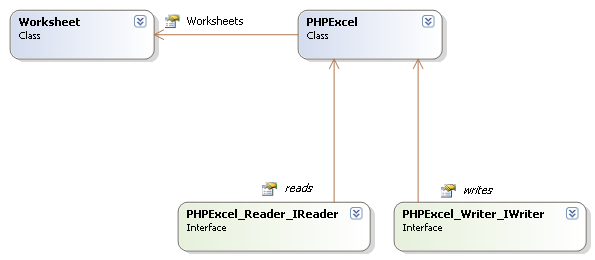
\includegraphics[scale=0.7]{skematik-phpexcel.png}  
	\caption[Arsitektur PHPExcel]{Arsitektur PHPExcel} 
	\label{fig:skematik-phpexcel} 
\end{figure}

Untuk menjalankan PHPExcel, diperlukan perangkat lunak sebagai berikut :
\begin{itemize}
	\item  PHP versi 5.2.0 keatas
	\item  PHP extension php\_zip enabled
	\item  PHP extension php\_xml diaktifkan
	\item  PHP extension php\_gd2 diaktifkan 
\end{itemize}


